\documentclass{article}
\usepackage[utf8]{inputenc}
\usepackage{hyperref}
\usepackage[letterpaper, portrait, margin=1in]{geometry}
\usepackage{enumitem}
\usepackage{amsmath}
\usepackage{booktabs}
\usepackage{graphicx}

\usepackage{titlesec}

\titleformat{\section}
{\normalfont\Large\bfseries}{\thesection}{1em}{}[{\titlerule[0.8pt]}]
  
\title{Homework 9}
\author{Ana Mazmishvili}
  
\begin{document}
  
\maketitle

\section{Stata}
\noindent 1.  A yearly plot of the recycling rate for NYC and the controls separately is presented on Figure \ref{fig:NYCNJMA}, while the sum of controls is presented on Figure \ref{fig:NYCvsControls}. 

\begin{figure}[h!]
    \centering
    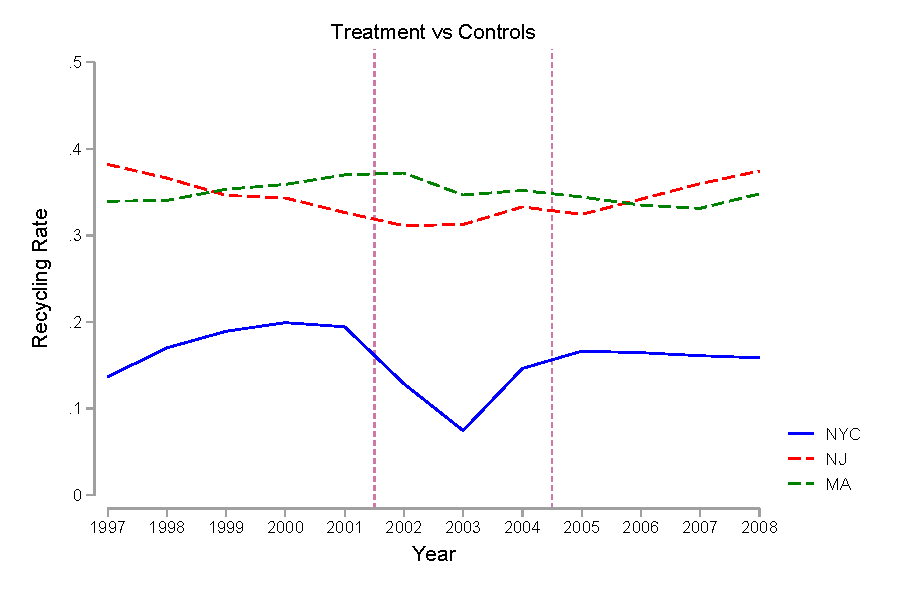
\includegraphics{homework 9/data/treatedvscontrol.pdf}
    \caption{Recycling rate for NYC and the controls}
    \label{fig:NYCNJMA}
\end{figure}

\begin{figure}[h!]
    \centering
    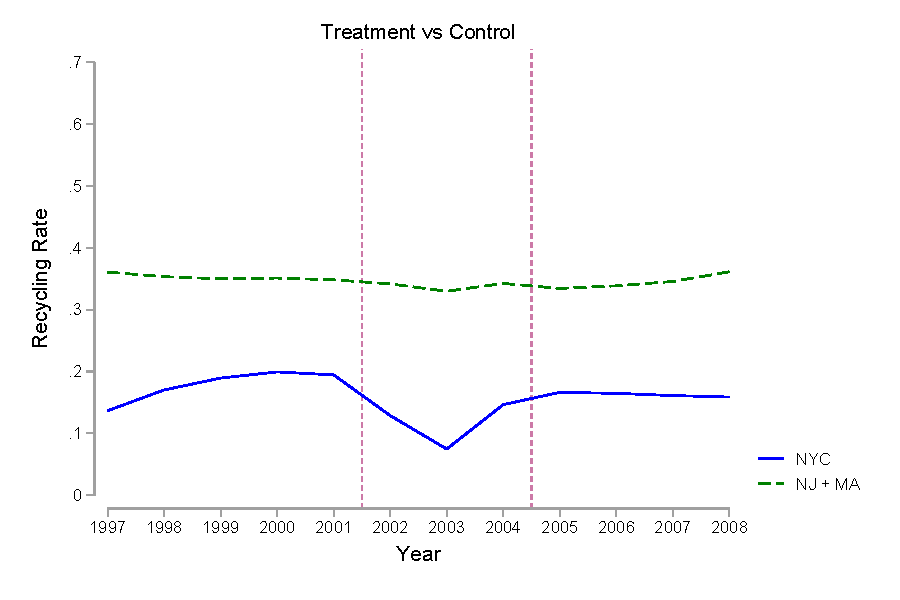
\includegraphics{homework 9/data/linechartrecyclingrate.pdf}
    \caption{Recycling rate for NYC and the sum of controls}
    \label{fig:NYCvsControls}
\end{figure}

\clearpage

\noindent 2. The effect of the pause on the recycling rate in NYC using a TWFE regression and the data
from 1997-2004 is  -.0619874 and the clustered standard error is  .0058221.


\noindent 3. The estimated average treatment effect and the synthetic DID is presented on the Fig ..

\noindent 4.  The event study regression results are presented on Fig 


\noindent 5.a The plot of raw outcomes for treated and control groups over time is presented on Fig 

\noindent 5.b. The plot of raw outcomes for treated group and synthetic control group over time is presented on Fig 

\noindent 5.c. The plot of estimated synthetic control effects and placebo effects over time is presented on Fig 

\noindent 5.d. The plot of final synthetic control estimates over time is presented on Fig 

\end{document}